\documentclass{beamer}
\usepackage[russian]{babel}
\usetheme{metropolis}

\usepackage{amsthm}
\setbeamertemplate{theorems}[numbered]

\setbeamercolor{block title}{use=structure,fg=white,bg=gray!75!black}
\setbeamercolor{block body}{use=structure,fg=black,bg=gray!20!white}

\usepackage[T2A]{fontenc}
\usepackage[utf8]{inputenc}

\usepackage{hyphenat}
\usepackage{amsmath}
\usepackage{graphicx}

\AtBeginEnvironment{proof}{\renewcommand{\qedsymbol}{}}{}{}

\title{
Микроэкономика-I
}
\author{
Павел Андреянов, PhD
}

\begin{document}

\maketitle

\section{Теорема об огибающей}

\begin{frame}{Теорема об огибающей}

Определим огибающую $V(p)$ как результат оптимизации функции $f$ по какому-то статическому множеству $Х$: 
$$ V(p) := \max_{x \in X} f(x, p),$$

\begin{theorem}[Об огибающей]
Функция $V(p)$ дифференциируема (почти всюду) и 
$$\frac{\partial V(p)}{\partial p} = \frac{\partial f(x, p)}{\partial p}|_{x = x^{\ast}(p)}.$$
\end{theorem}

... то есть, наклон огибающей (в пространстве параметров) равен наклону опорной функции в точке касания.

\end{frame}

\begin{frame}{Теорема об огибающей}

Рассмотрим простой пример:

Опорная функция $$ f(x|a,b) = - (x-a)^2 - b $$
Максимизируем ее $$ x^{\ast} = a, \quad f^{\ast} = - b $$
Дифференциируем истинный ответ: $$\partial f^{\ast}/\partial a = 0, \ \partial f^{\ast}/\partial b = -1$$
Дифференциируем (казалось бы, зачем?) опорную функцию: $$\partial f/\partial a = -2(x^{\ast}-a), \ \partial f/\partial b = -1$$
\end{frame}

\section{Минимизация расходов}

\begin{frame}{Минимизация расходов}

Для простоты пусть будут два товара $x, y$ с ценами $p, q$.

Классическая задача максимизации полезности:
$$\text{P1:} \quad U(x, y) \to \max_{x,y \geqslant 0}, \quad \text{s.t.} \quad p x + q y \leqslant W.$$

Дуальная (к ней) задача минимизации расходов:
$$\text{P2:} \quad p x + q y \to \min_{x,y \geqslant 0}, \quad \text{s.t.} \quad U(x,y) \geqslant \bar U.$$

\end{frame}

\begin{frame}{Минимизация расходов}

Решение задачи (P1) максимизации полезности это так называемые маршаллианские спросы $m_x(p,q,W)$, $m_y(p,q,W)$ и косвенная полезность $V(p,q,W)$.

Решение задачи (P2) минимизации расходов это так называемые хиксианские спросы $h_x(p,q,\bar U)$, $h_y(p,q,\bar U)$ и функция расходов $E(p,q,\bar U)$.

\end{frame}

\begin{frame}{Минимизация расходов}
Сравним лагранжианы
\begin{gather*}
\mathcal{L}^{1} = U(x, y) - \lambda (px + qy - W)\\
\mathcal{L}^{2} = (px + qy - W) - \gamma (\bar U - U(x,y))
\end{gather*}

Сравним фоки (упп)
\begin{gather*}
\text{P1:} \quad U'_x = \lambda p, \quad U'_y = \lambda q, \quad px + qy = W\\
\text{P2:} \quad p = \gamma U'_x, \quad q = \gamma U'_y, \quad U(x,y) = \bar U
\end{gather*}

Решения совпадают, если третьи уравнения эквивалентны.

\end{frame}

\section{Закон Вальраса}

\begin{frame}{Закон Вальраса}

\begin{theorem}[Закон Вальраса]
Если полезность локально ненасыщаема в $\mathbb{R}^n_{+}$, то любое из решений задачи максимизации полезности всегда лежит на бюджетном ограничении.
\end{theorem}

Это утверждение доказывается от противного. 

\end{frame}

\section{Дуальность}

\begin{frame}{Дуальность}

Мы подошли к очень важному наблюдению.

\begin{theorem}[Дуальность]

Если полезность (квази-)вогнутая и локально ненасыщаемая, то любое решение (как функция от цен) задачи минимизации расходов воспроизводится как одно из решений максимизации полезности и наоборот.
\end{theorem}
Причем, все это при одних и тех же ценах. Это чуть более сильное утверждение чем просто закон Вальраса. 

\end{frame}

\begin{frame}
Это значит, что задача максимизации полезности и задача минимизации расходов по большому счету эквивалентны в определенном геометрическом смысле. 

Более того, для того чтобы понять при каком уровне полезности $\bar U$ решение задачи минимизации расходов совпадет с решением задачи максимизации полезности при бюджете $W$, надо положить $$\bar U := V(p,q,W),$$ и тогда вы потратите в точности $W$.

\end{frame}

\begin{frame}

То есть, для любых цен верно что $$\bar U = V(p, q, E(p,q, \bar U)), \quad W = E(p,q, V(p,q,W)).$$
и верно что
$$ h = m(p, q, E(p,q, \bar U)), \quad m = h(p,q, V(p,q,W)$$
\end{frame}

\section{Тождество Роя}

\begin{frame}{Тождество Роя}

Воспользуемся дуальностью:
$$U = V(p, q, E(p,q,U)).$$
Убедитесь, что это действительно корректная запись.

Что можно сделать с этим тождеством?
\begin{itemize}
\item продифференцировать по $p$
\item продифференцировать по $q$
\end{itemize}
ведь оно выполнено при всех $p,q$.

\end{frame}

%%%%%%%%%%%%%%%%

\begin{frame}{Тождество Роя}
Заметим, что цены входят справа дважды:
$$\bar U = V(p, q, E(p,q, \bar U)).$$
По правилам дифференцирования, полный дифференциал функции $V$ по $p$ равен:
\begin{gather*}
\frac{d V}{d p} = \frac{\partial V}{\partial p} + \frac{\partial V}{\partial W} \cdot \frac{\partial E}{\partial p} = 0
\end{gather*}
Все это при заданном $\bar U$ и меняющихся ценах.
\end{frame}

\begin{frame}{Тождество Роя}
Поскольку $\frac{\partial E}{\partial p} = h$, 
$$\frac{d V}{d p} = \frac{\partial V}{\partial p} + \frac{\partial V}{\partial W} \cdot h_x = 0$$
Aналогично для второй цены
$$\frac{d V}{d q} = \frac{\partial V}{\partial q} + \frac{\partial V}{\partial W} \cdot h_y = 0$$
Вспоминая что $m = h$ получаем:

\begin{theorem}[Тождество Роя]
Если $\vec{m}$ - весь вектор спросов, а $\vec{p}$ - весь вектор цен то
$$\vec{m} = - \frac{\nabla_{\vec{p}} V}{\partial V / \partial W } $$
\end{theorem}

\end{frame}

\section{Как не запутаться?}

\begin{frame}{Как не запутаться?}

Подводя итог, у нас было две задачи: максимизации полезности и минимизации расходов.
Каждая задача произвела три обьекта:

\begin{itemize}
\item оптимальные $m_x(p,q,W), m_y(p,q,W)$ и косвенная полезность $V(p,q,W)$ в первой задаче
\item оптимальные $h_x(p,q,\bar U), h_y(p,q,\bar U)$ и функция расходов $E(p,q,\bar U)$ во второй задаче
\end{itemize}
Можно изобразить <<схему перемещений>> между объектами

\end{frame}

\begin{frame}{Как не запутаться?}

\begin{figure}[hbt]
\centering
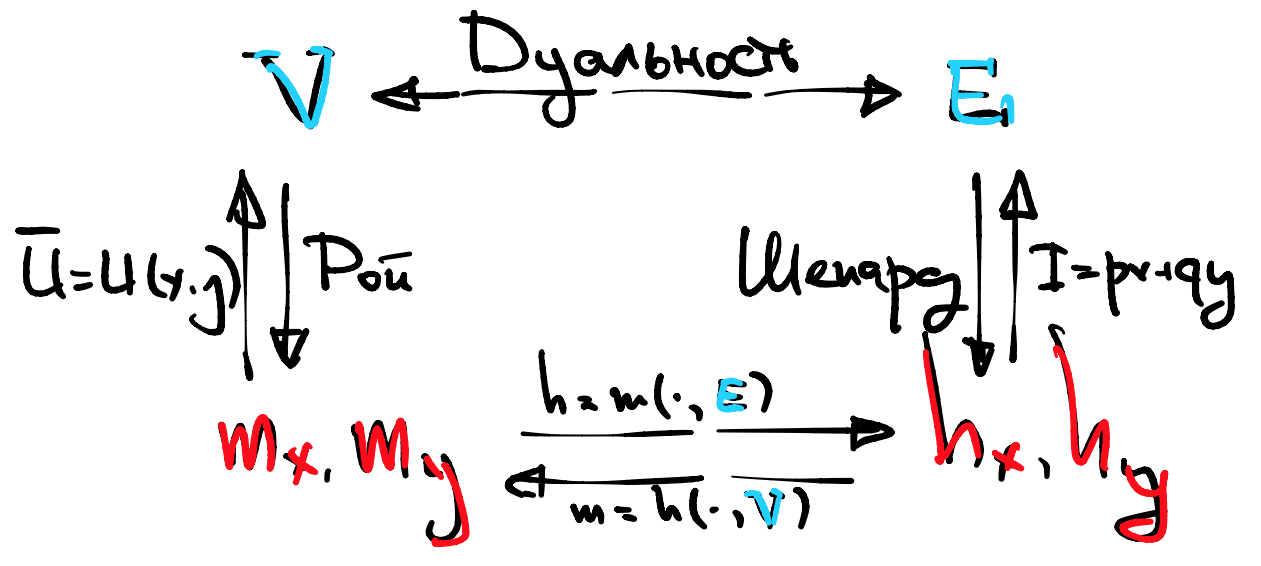
\includegraphics[width=.9\textwidth]{scheme.png}
\end{figure}

\end{frame}

\section{Примеры на доске}

\end{document}